\chapter{Event Reconstruction}
\label{reconstruction_chapter}

\section{Electron Reconstruction}
\label{sec:electron_reconstruction}

Reconstruction of electrons in CMS is complicated by the fact that electrons,
because of their low mass and the high magnetic field, emit photon which must
be accounted for in the final energy sum. Additionally, the amount of material
in front of ECAL causes many electrons begin showering before entering ECAL,
adding additional scattered energy deposits that must be included in the final
sum. Information about the material in front of ECAL is given in
\FIG~\ref{fig:tracker_material}\cite{cms_tracker_2014}.

\begin{figure}[!htbp]
    \centering
    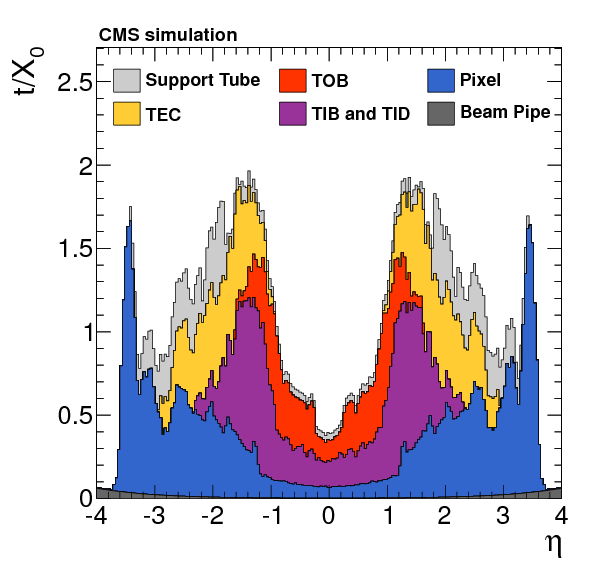
\includegraphics[width=\textwidth]{figures/tracker_material_budget.png}
    \caption[
        Material thickness infront of of ECAL.
    ]{
        The thickness of material, $t$, divided by the radiation length,
        \radiationlength, encountered by particles leaving the nominal
        interaction point before reaching ECAL.
    }
    \label{fig:tracker_material}
\end{figure}

The reconstruction of electrons with $\pt > 20 \GeV$ in CMS starts with an
electron-like cluster of energy in ECAL \cite{eg_reco_2010}. In order to
account for energy lost to photon radiation, additional clusters at constant
$\eta$ but changing $\phi$ are added together to form superclusters
\cite{baffioni_2007}. \TODO{A bit about how various deposits of energy are
connected to form the supercluster.}

From these superclusters, a volume in the tracker where the electron is likely
to have come from is determined by propagating the energy weighted mean
position of the supercluster back through the magnetic field. This spot is then
used to seed  track finding algorithm in the pixel layer. Hits in the tracker
are searched from starting at the innermost layer and working outward. In order
to account for the changing shape of the track as the electron loses energy
from interacting with the tracker material, a ``Gaussian Sum Filter'' (GSF)
\cite{adam_2005} is used rather than the simpler Kalman filter used for muons
and hadrons. Low energy electrons ($\ET < 15 \GeV$) are constructed with \pt
from the tracker and \ET from ECAL. For higher energy electrons, the ECAL
energy is used without the tracker \pt to avoid issues introduced by the
possible poor fits in the tracker. The $\eta$ and $\phi$ of all electron
candidates, regardless of energy, is taken from the track by projecting back to
the interaction point.

\section{Additional Corrections}

Although the measurement of \phistar is insensitive to the energy of the
electrons, the energy still plays a role in determining the electron \pt and
hence whether an event passes the selection criteria used in this analysis
(discussed in \SEC~\ref{ssec:electron_selection}). Therefore, it is important
to accurately measure this quantity, even if it does not directly effect the
final observable. To this end, two sets of centrally produced electron energy
and momentum corrections are applied to both the data and the reconstructed MC
quantities.

\subsection{Regression}

The first set of corrections were calculated using a multivariate regression
trained on \Ztoee and \higgstoZZ MC \cite{cms_an_2012-327}. The regression used
a boosted decision tree trained on 41 different variables parameterizing
electron shower shape, the electron track, and the location of the shower in
EB. The algorithm was trained separately for EB and EE electrons. In order to
prevent over-training the MC samples were split in half, with one half used for
training and the other half used for validation. Electrons used in the
regression were required to have low radiated energy fraction ($< 0.01$) as
determined by the generator level MC and $\pt > 7 \GeV$. The target variable
was the ratio of the gen level bare electron energy over the reconstructed
energy. This correction was applied to both the data and the reconstructed MC
electrons used in this analysis.

\subsection{Energy Scale and Resolution}

The second set of corrections were calculated with \Ztoee MC using two
independent methods \cite{cms_an_2013-253}. The first method was used to
correct for the energy scale while the second method was used to correct for
the resolution.

In the first method, the MC sample and the data were fit with the convolution
of a Breit-Wigner with a Crystal Ball (CB) function. The CB function is used to
model the resolution of the detector and losses due to bremsstrahlung from the
material in front of ECAL. It consists of a Gaussian with a power-law low-side
tail. It was first used by the Crystal Ball Collaboration \cite{oreglia_1980}.
The Breit--Wigner function models the analytic shape predicted for the \Z mass
resonance. The parameters of the Breit--Wigner were fixed to the nominal values
from the Particle Data Group: $\MZ = 91.188 \GeV$, $\GammaZ = 2.495 \GeV$. The
parameters of the CB function were free parameters in the fit.

The scale correction is both time dependent and $\eta$ dependent and so fits
were performed separately in four pseudorapidity bins in various run ranges.
The peak of the CB function in data and MC were compared with the relative
shift taken as the scale correction, $\Delta P$, given by
\EQ~\ref{eq:scale_correction}.

\begin{equation} \label{eq:scale_correction}
    \Delta P = \frac{\Delta m_{\text{data}} - \Delta m_{\text{MC}}}{\MZ}
\end{equation}

In the second method, two categories of electrons are defined: showering
electrons ($\RNine < 0.94$) and non-showering electrons ($\RNine > 0.94$). A
probability density function (PDF) is created using the \Ztoee MC. For each
event in the PDF, the supercluster energy is modified by applying a Gaussian
multiplicative factor $1+\Delta P$ with a standard deviation of $\Delta \sigma$,
where $\Delta P$ is the scale correction and $\Delta \sigma$ models the
resolution. The resolution parameter was selected for each of the two types of
electrons, the four pseudorapidity bins, and various run ranges using a
likelihood maximization. In the EB pseudorapidity bins, there were enough
events to bin in \ET and so these corrections are also \ET dependent.

\section{Electron Variables}
\label{sec:electron_variables}

Reconstructed electrons have multiple variables that indicate their quality.
These variables are broken down into three main categories:

\begin{description}
    \item[Isolation:] \hfill \\
        These variables measures how much energy from other particles is
        deposited near the electron in the detector and are used to help reject
        jets.
    \item[Identification (ID):] \hfill \\
        These variables quantify how much like an electron the reconstructed
        particle looks and are used to reject pions and other charged
        particles.
    \item[Conversion Rejection:] \hfill \\
        These variables are used to reject electrons from \photontoee
        conversions.
\end{description}

\subsection{Isolation}

Hadronic jets sometimes produce electrons in the numerous decays happening
within them. These electrons can be rejected by looking at the sum of the
energy in the tacker, ECAL, and HCAL around the electron, as electrons in jets
will have a large amount of energy surrounding them, whereas electrons from \Z
decays will tend to be isolated.

The isolations used in the trigger (\SingleElectronTrigger) are defined as
follows:

\begin{equation}
    \HCALISO = \DeltaRSum \EHCAL
\end{equation}

\begin{equation}
    \ECALISO = \DeltaRSum \EECAL - \ESC
\end{equation}

Where \DeltaRSum is a sum on the energy in a $\Delta R < 0.3$ cone around the
supercluster location, \EHCAL is the energy in HCAL, \EECAL is the energy in
ECAL, and \ESC is the energy of the supercluster, which is subtracted out of
the ECAL isolation sum. No subtraction is applied to the HCAL isolation as we
expect all of the electron's energy to be contained in ECAL.

A different isolation variable is defined for offline selection that is more
expensive to compute but takes advantage of the tracker as well as ECAL and
HCAL. This isolation uses a \particleflow\cite{particle_flow_2010} technique
which is a method of reconstructing jets that uses information for every
subdetector and tries to reconstruct the individual particles in a jet by
matching them to their responses in the various subdetectors. To keep the
algorithm simple, \particleflow categorizes every particle into one of five
types: photons, electrons, muons, charged hadrons, and neutral hadrons. A
photon is a particle with energy only deposited in ECAL. An electron is a
particle with an ECAL energy deposit and a track. A muon is a track in the
central tracker matched to a track in the muon system. A charged hadron is any
energy cluster in HCAL with a matching ECAL cluster and track. A neutral hadron
is any energy cluster in HCAL with a matching ECAL cluster without a matching
track. These particle flow jets are used to calculate an energy per area due to
pileup, $\rho$, in the detector which is used to remove the pileup contribution
from the isolation sum. The \particleflow isolation, $\PFISO$, is given by:

\begin{equation}
    \PFISO = \DeltaRSum \left(\ptTrack + \EECAL + \EHCAL\right) - \ptElectron
    - \ESC - 0.3^{2} \pi \rho
\end{equation}

Where the variables are the same as above, with the addition of \ptTrack, which
is the \pt of all tracks in the tracker, \ptElectron, which is the \pt of the
electron's track, and $\left(0.3^{2} \pi \rho\right)$, which is the energy
around the electron calculated from particle flow. A comparison of the
distribution of \PFISO in a minimally biased ensemble of electrons from events
selected with a muon trigger and the same distribution in the \MADGRAPH signal
sample is shown in \FIG~\ref{fig:pf_iso}; a similar comparisons distributions
of \HCALISO and \ECALISO are shown in \FIGS~\ref{fig:hcal_iso} and
\ref{fig:ecal_iso}.

\begin{figure}[!htbp]
    \centering
    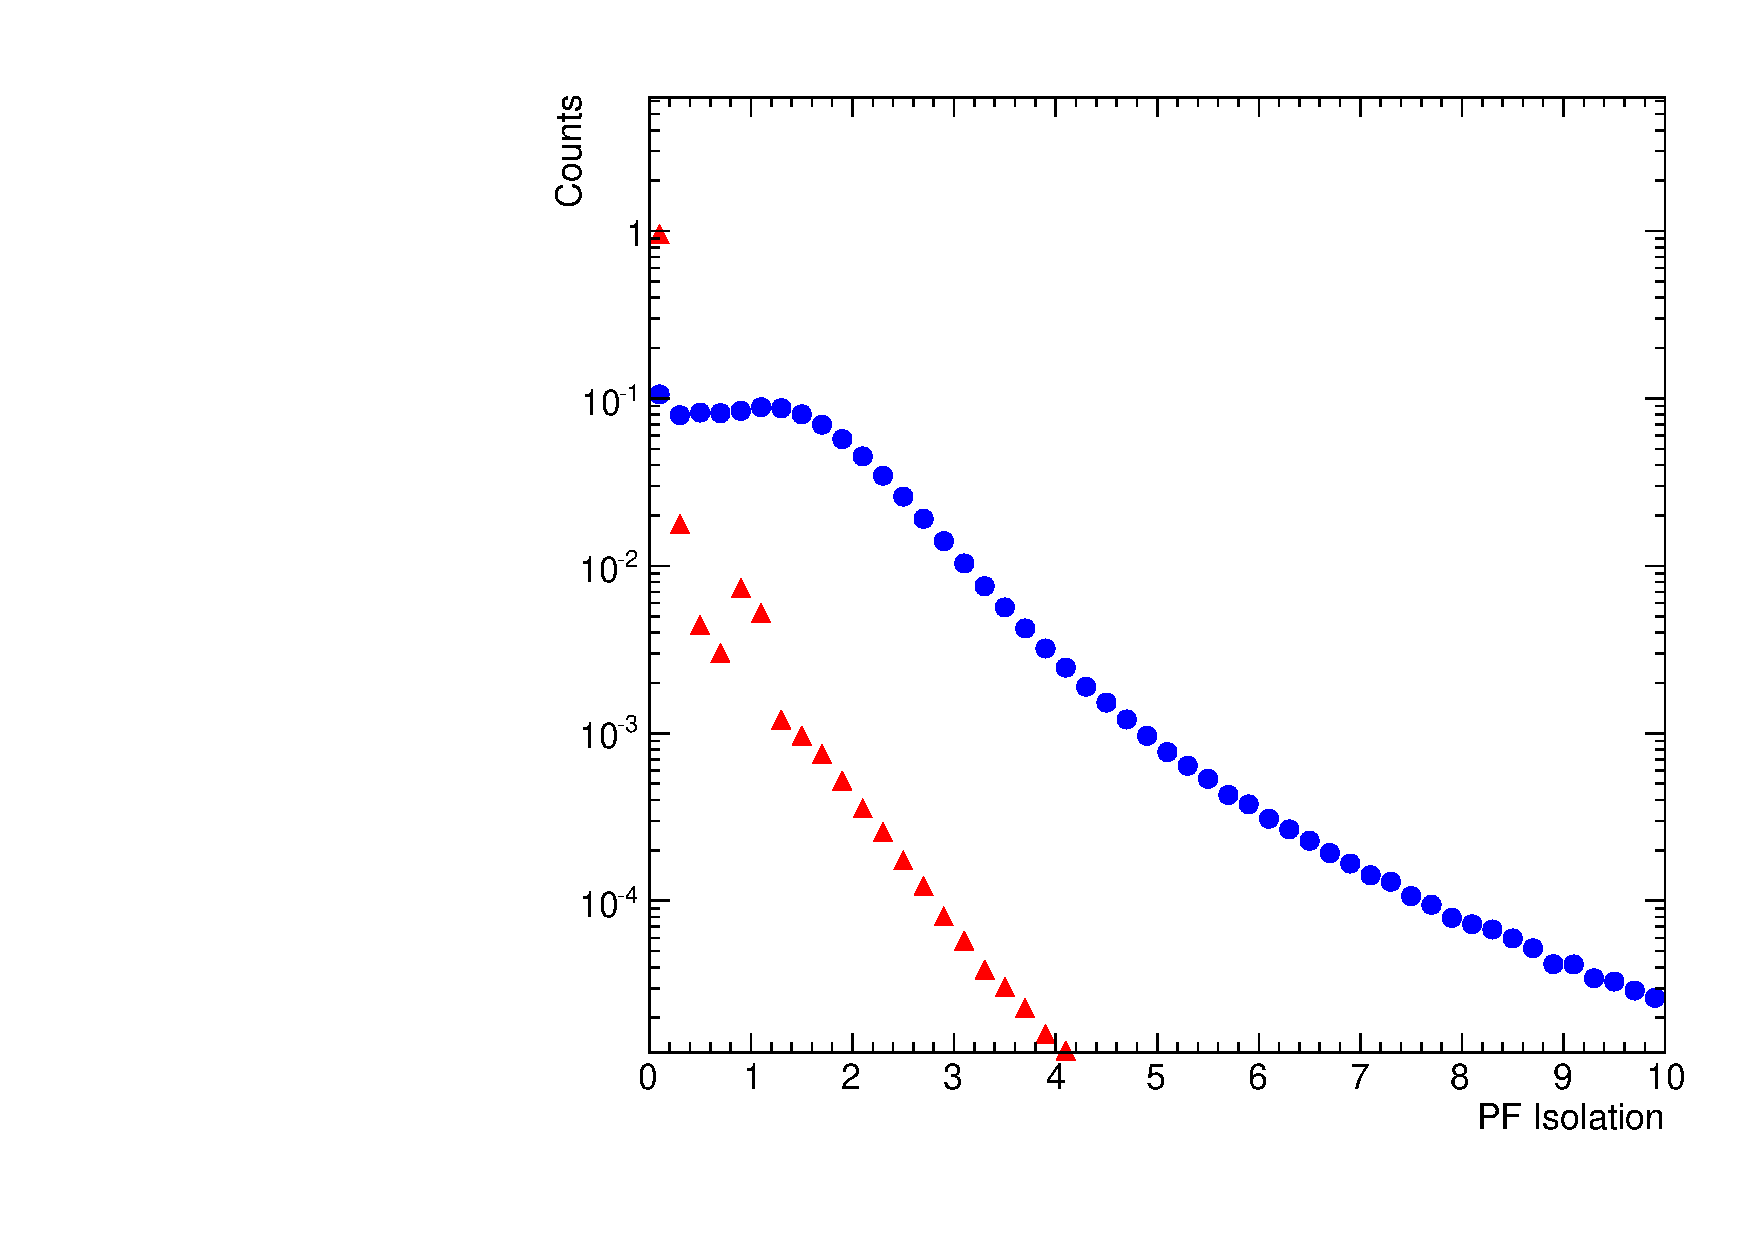
\includegraphics[width=0.65\textwidth]{figures/iso.pdf}
    \caption[
        Distributions of particle flow isolation variables in data and MC.
    ]{
        The particle flow isolation variable distribution for all electrons
        with $\pt > 20 \GeV$ and $|\eta| < 2.4$ in a set of events selected
        with a muon trigger (circles) and in \MADGRAPH \Ztoee MC (triangles).
    }
    \label{fig:pf_iso}
\end{figure}

\begin{figure}[!htbp]
    \centering
    \begin{subfigure}[b]{0.65\textwidth}
        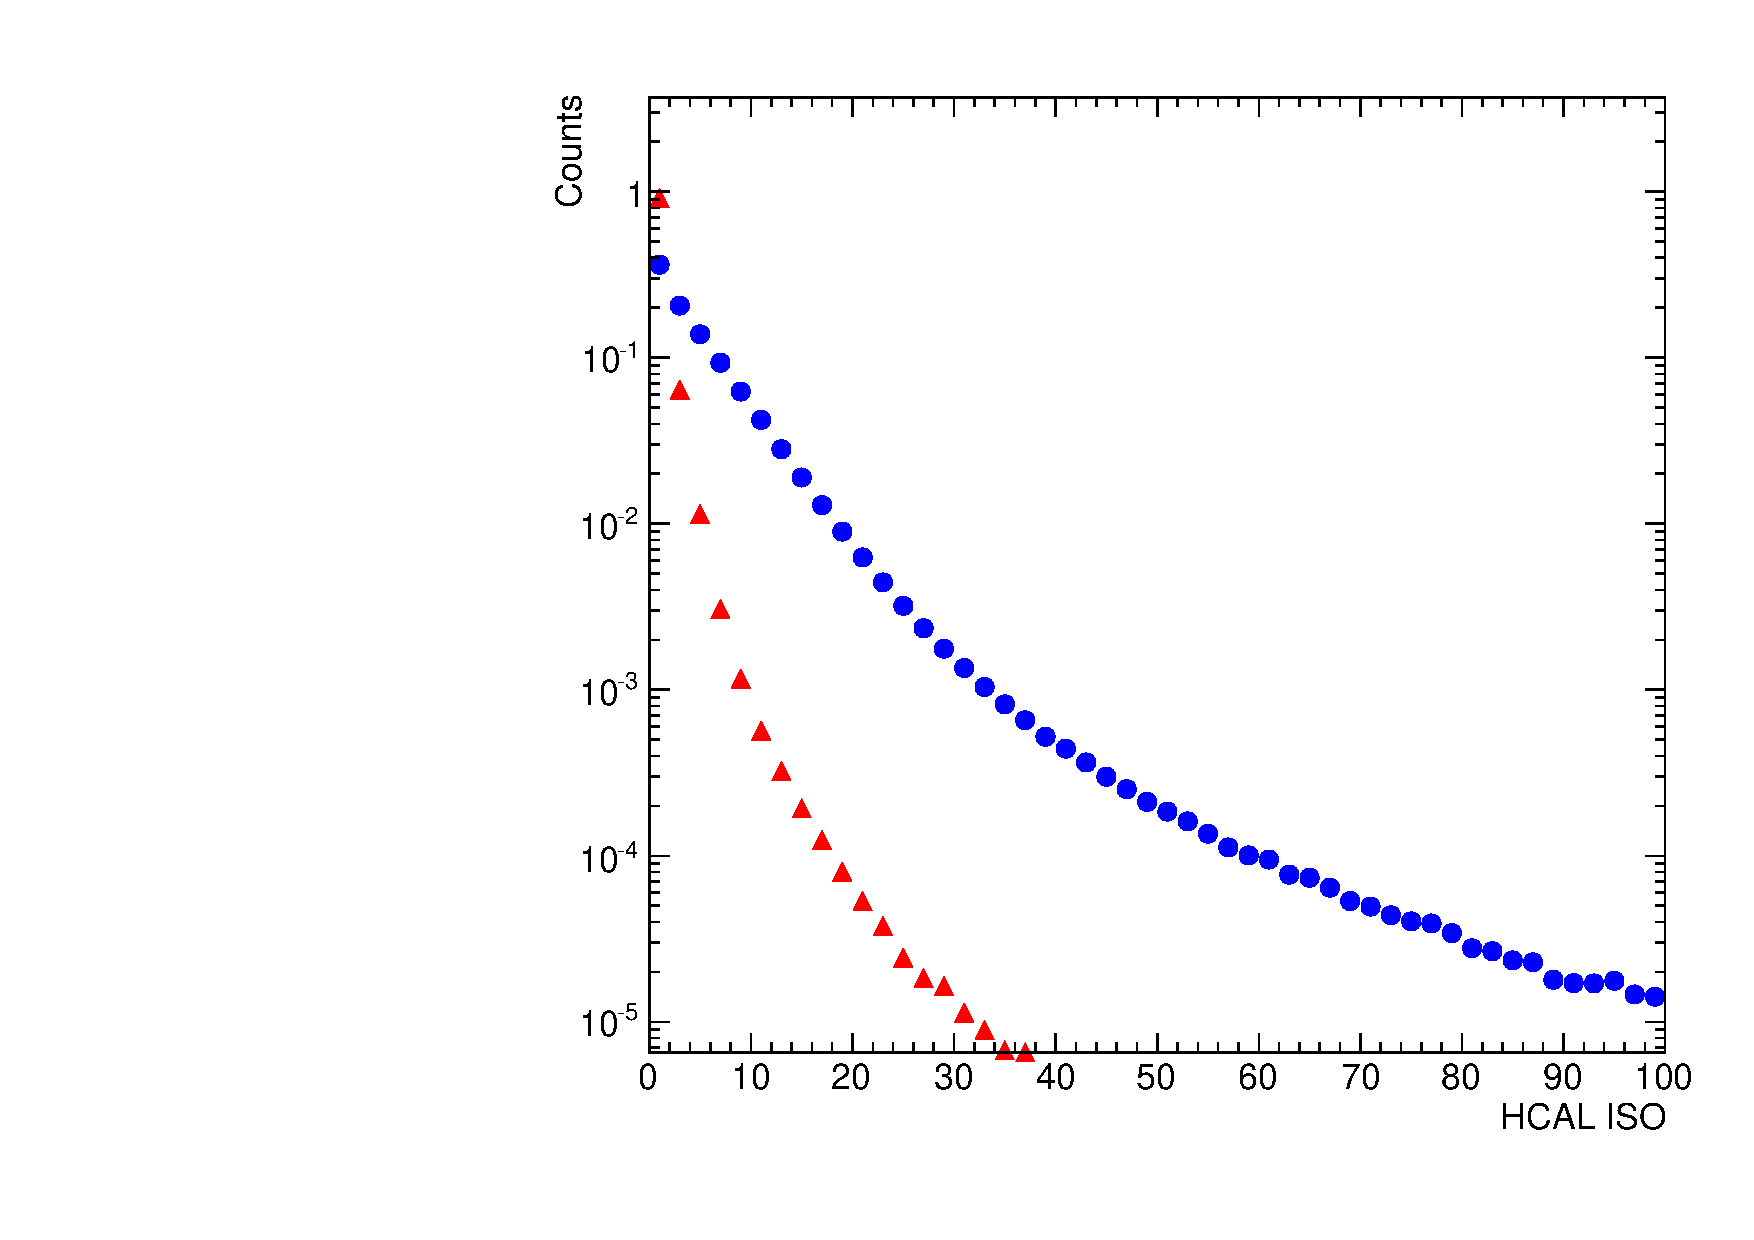
\includegraphics[width=\textwidth]{figures/hcal_iso.pdf}
        \caption{}
        \label{fig:hcal_iso}
    \end{subfigure}
    \begin{subfigure}[b]{0.65\textwidth}
        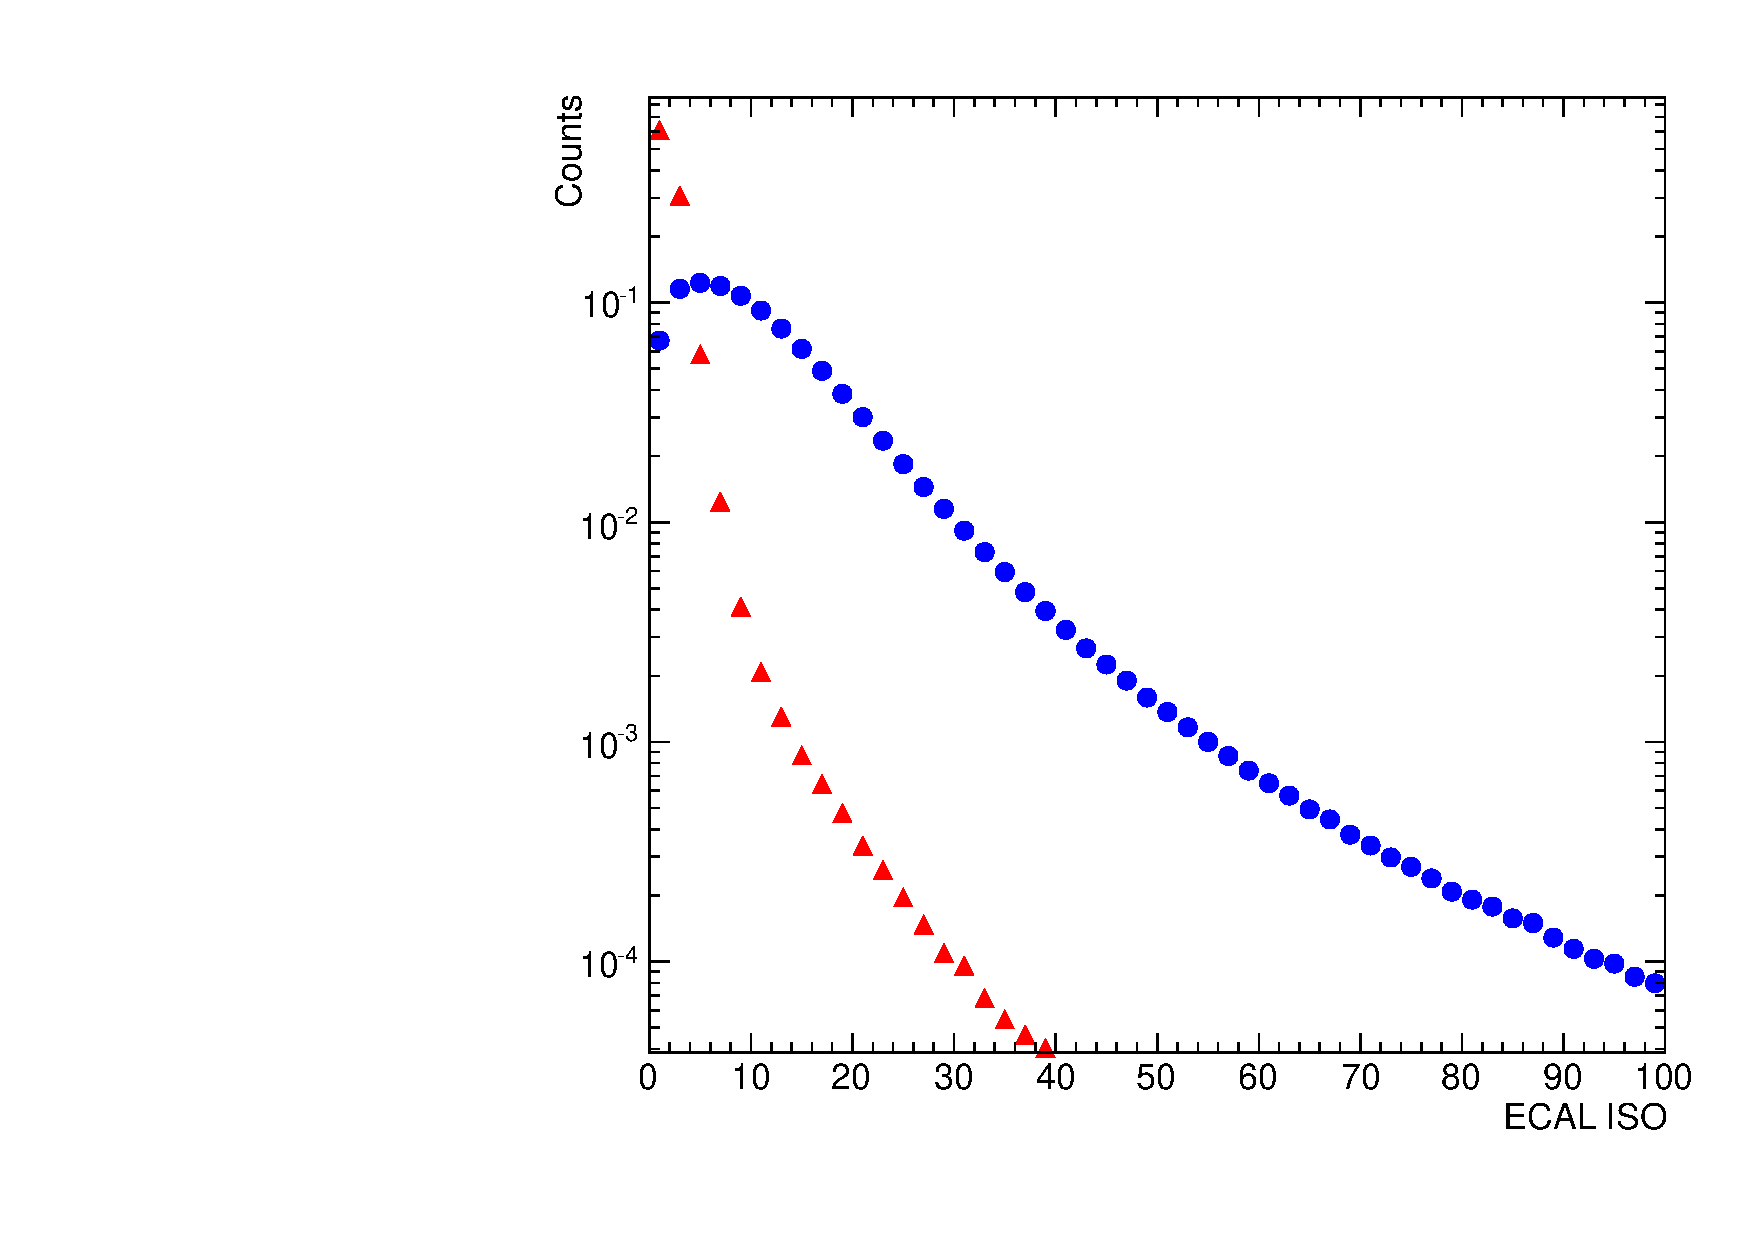
\includegraphics[width=\textwidth]{figures/ecal_iso.pdf}
        \caption{}
        \label{fig:ecal_iso}
    \end{subfigure}
    \caption[
        Distributions of HCAL and ECAL isolation variables in data and MC.
    ]{
        The HCAL (top) and ECAL (bottom) isolation variable distributions for
        all electrons with $\pt > 20 \GeV$ and $|\eta| < 2.4$ in a set of
        events selected with a muon trigger (circles) and in \MADGRAPH \Ztoee
        MC (triangles).
    }
    \label{fig:hcal_ecal_isos}
\end{figure}

\subsection{Identification}

The shape of the electromagnetic shower in the calorimeters is used to
discriminate between electrons and other particles. Electrons generally have
very narrow showers whereas hadronic particles have wide showers. The size of
the shower in $\eta$ is characterized by \sigmaietaieta. Electron showers are
mostly contained within ECAL and so the ratio of energy around the hit in HCAL
over the energy around the hit in ECAL, \HOverE, is also used to parameterize
the shower shape.

The distance between the track and the supercluster in \coordetaphi space is
given by \dphiin and \detain. The compatibility of energy of the supercluster
and the momentum of the track is parameterized by \ooeoop. Using these
variables photons can be rejected as they interact in ECAL but leave no track
in the tracker. A comparison of the distribution of $\HOverE$ is shown in
\FIG~\ref{fig:he}; compairisons of the distributions of $\sigmaietaieta$ and of
$\ooeoop$ are shown in \FIGS~\ref{fig:sieie} and \ref{fig:ooeoop}; comparisons
of the distributions of $\detain$ and $\dphiin$ are shown in
\FIGS~\ref{fig:deta} and \ref{fig:dphi}.

\begin{figure}[!htbp]
    \centering
    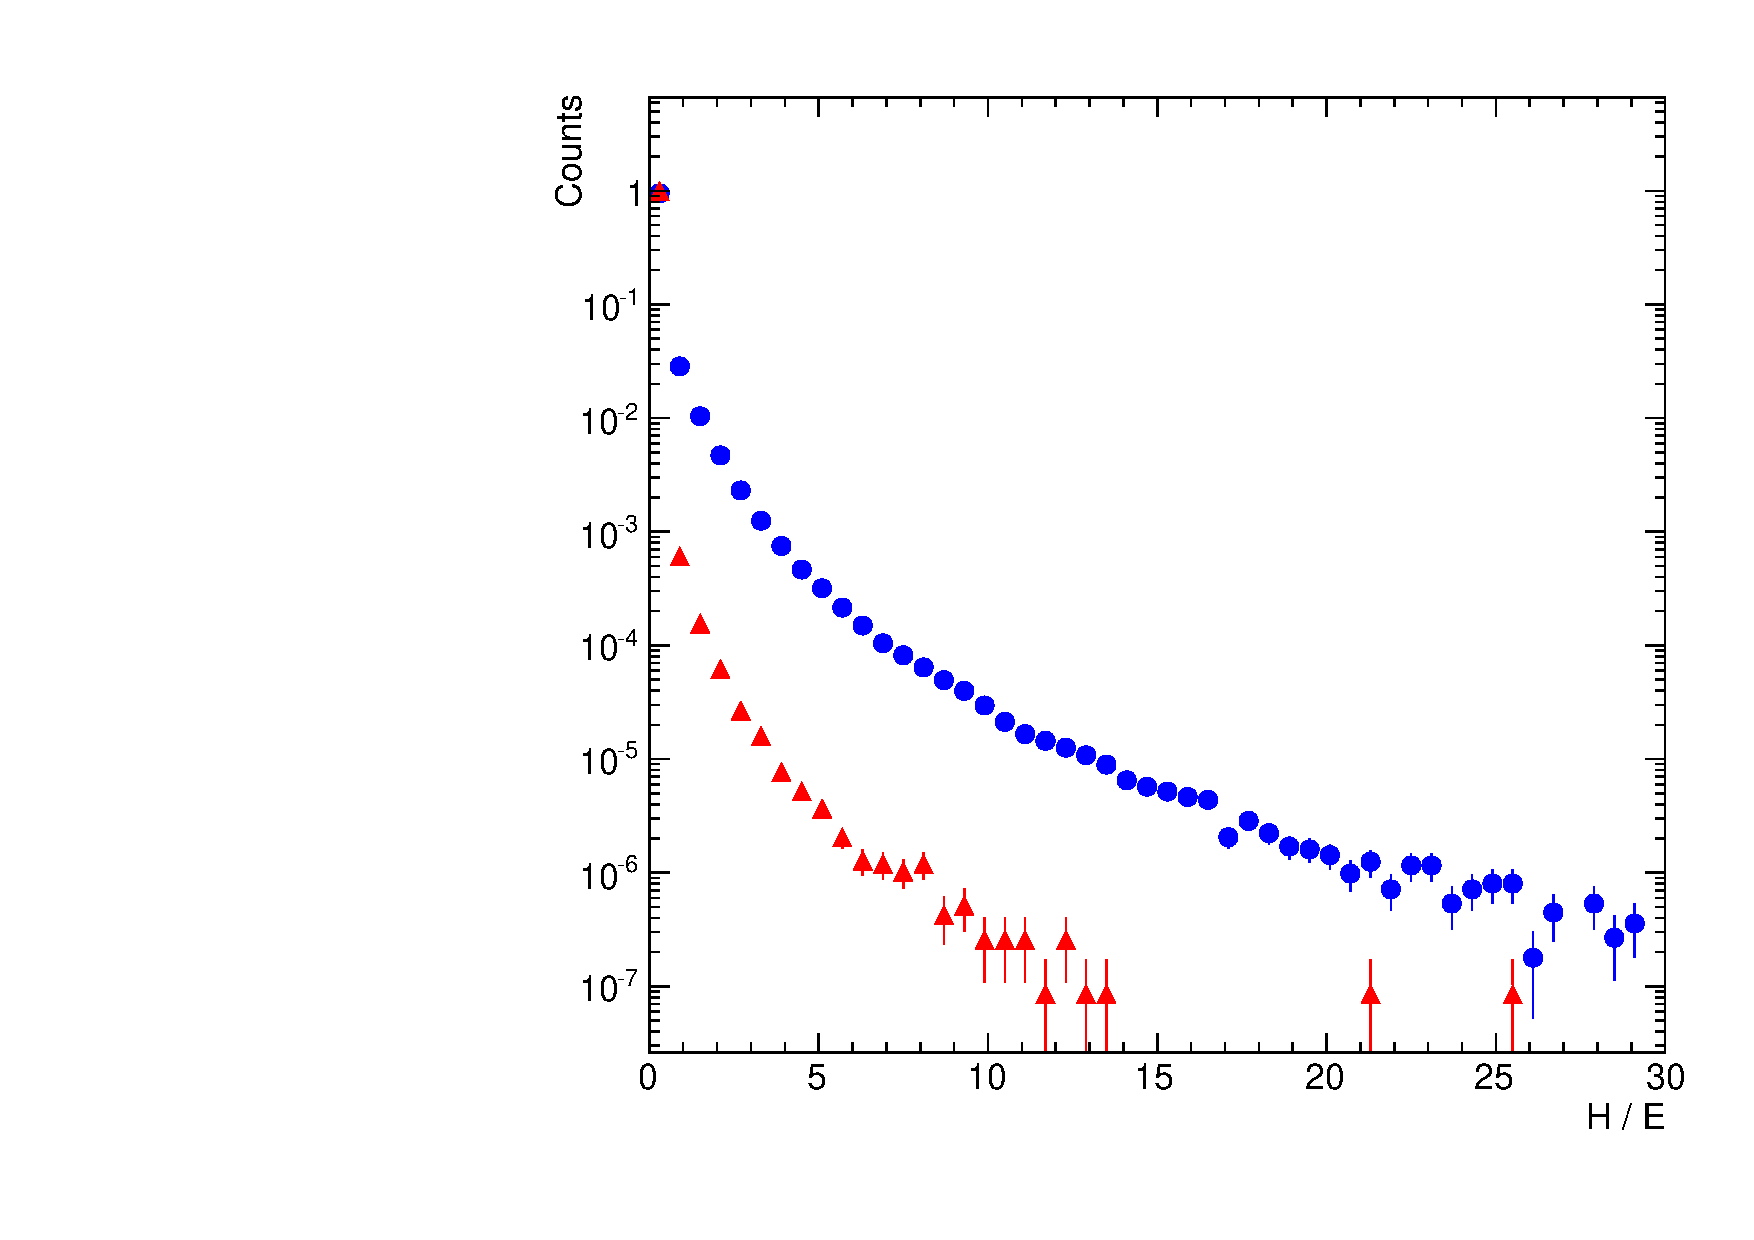
\includegraphics[width=0.65\textwidth]{figures/he.pdf}
    \caption[
        Distributions of \HOverE variable in data and MC.
    ]{
        The \HOverE variable distribution for all electrons with $\pt > 20
        \GeV$ and $|\eta| < 2.4$ in a set of events selected with a muon
        trigger (circles) and in \MADGRAPH \Ztoee MC (triangles).
    }
    \label{fig:he}
\end{figure}

\begin{figure}[!htbp]
    \centering
    \begin{subfigure}[b]{0.65\textwidth}
        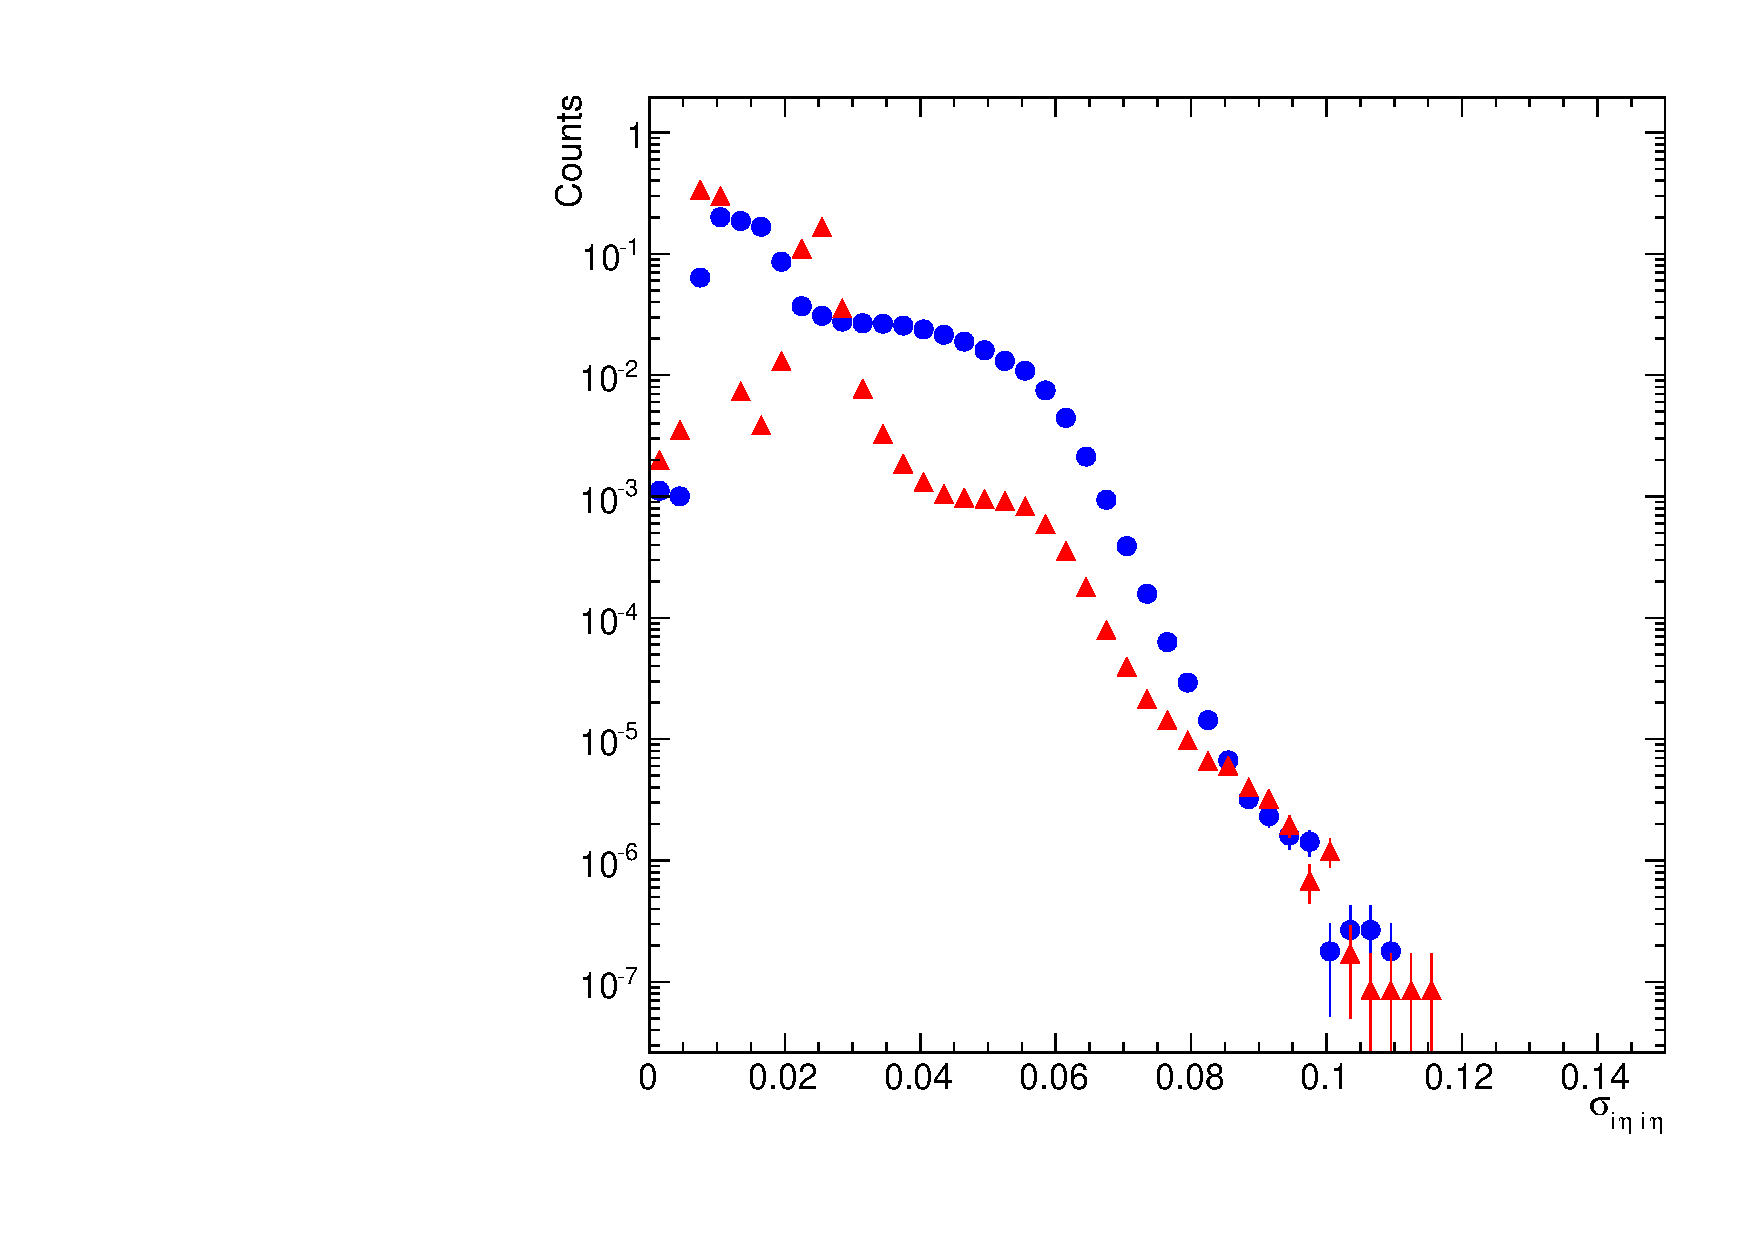
\includegraphics[width=\textwidth]{figures/sigma_ieta_ieta.pdf}
        \caption{}
        \label{fig:sieie}
    \end{subfigure}
    \begin{subfigure}[b]{0.65\textwidth}
        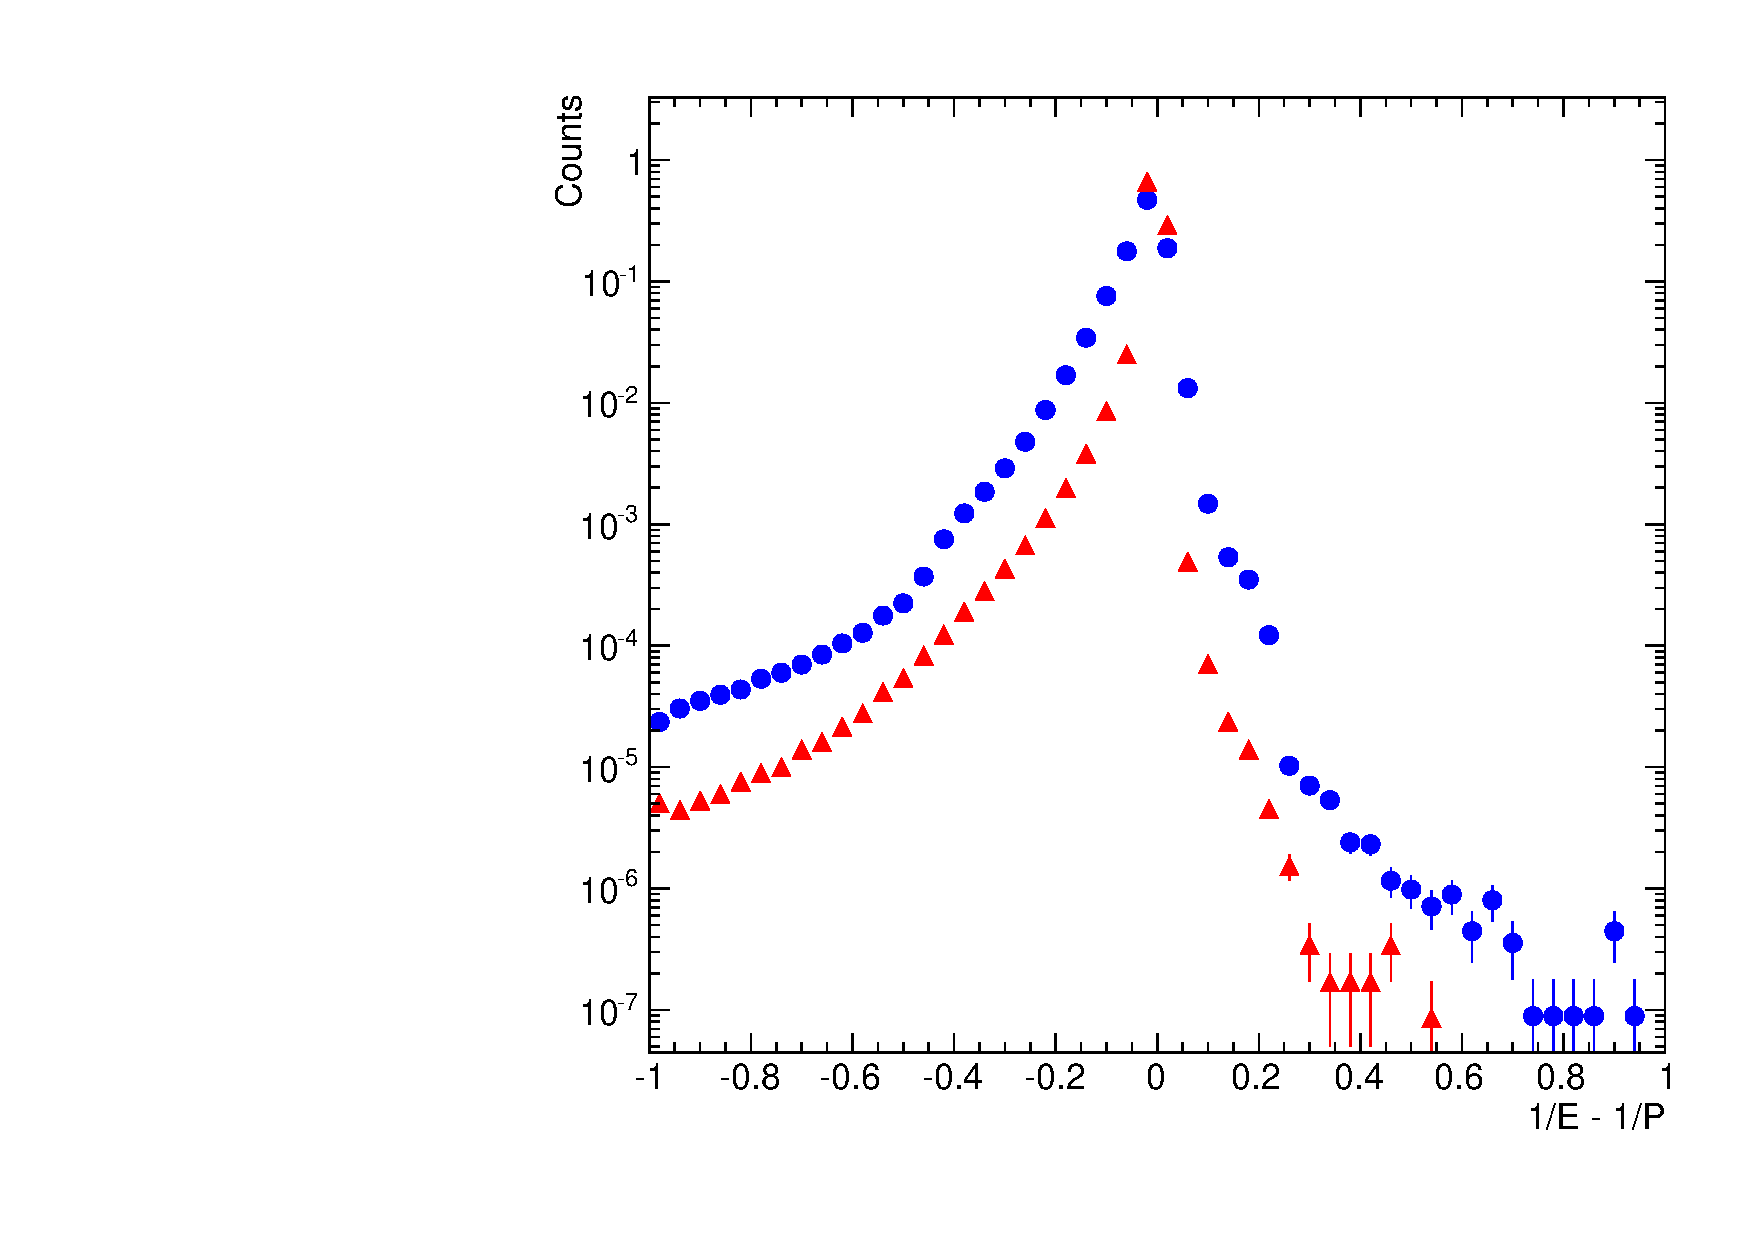
\includegraphics[width=\textwidth]{figures/1oe_1op.pdf}
        \caption{}
        \label{fig:ooeoop}
    \end{subfigure}
    \caption[
        Distributions of $\sigmaietaieta$ and $\ooeoop$ in data and MC.
    ]{
        The $\sigmaietaieta$ (top) and $\ooeoop$ (bottom) variable
        distributions for all electrons with $\pt > 20 \GeV$ and $|\eta| < 2.4$
        in a set of events selected with a muon trigger (circles) and in
        \MADGRAPH \Ztoee MC (triangles).
    }
    \label{fig:sieie_ooeoop}
\end{figure}

\begin{figure}[!htbp]
    \centering
    \begin{subfigure}[b]{0.65\textwidth}
        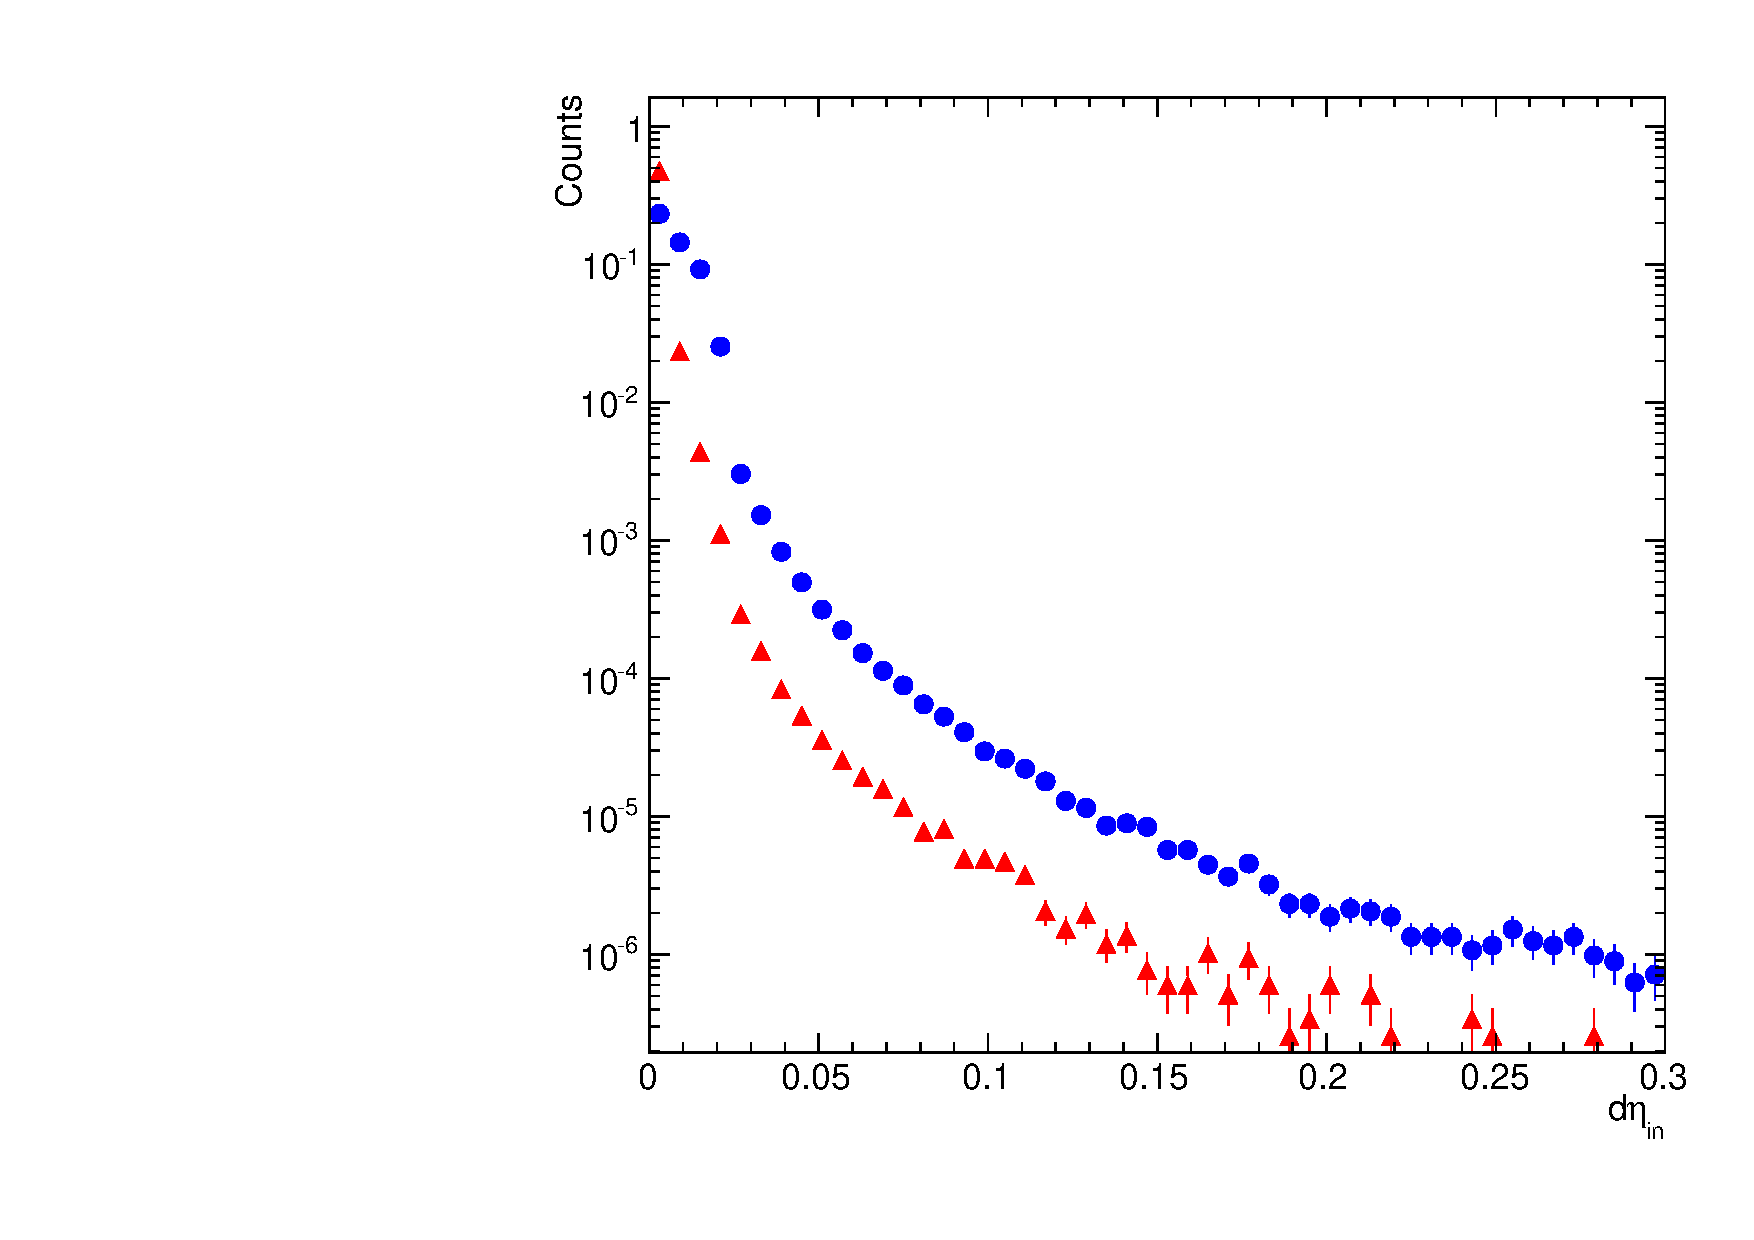
\includegraphics[width=\textwidth]{figures/deta.pdf}
        \caption{}
        \label{fig:deta}
    \end{subfigure}
    \begin{subfigure}[b]{0.65\textwidth}
        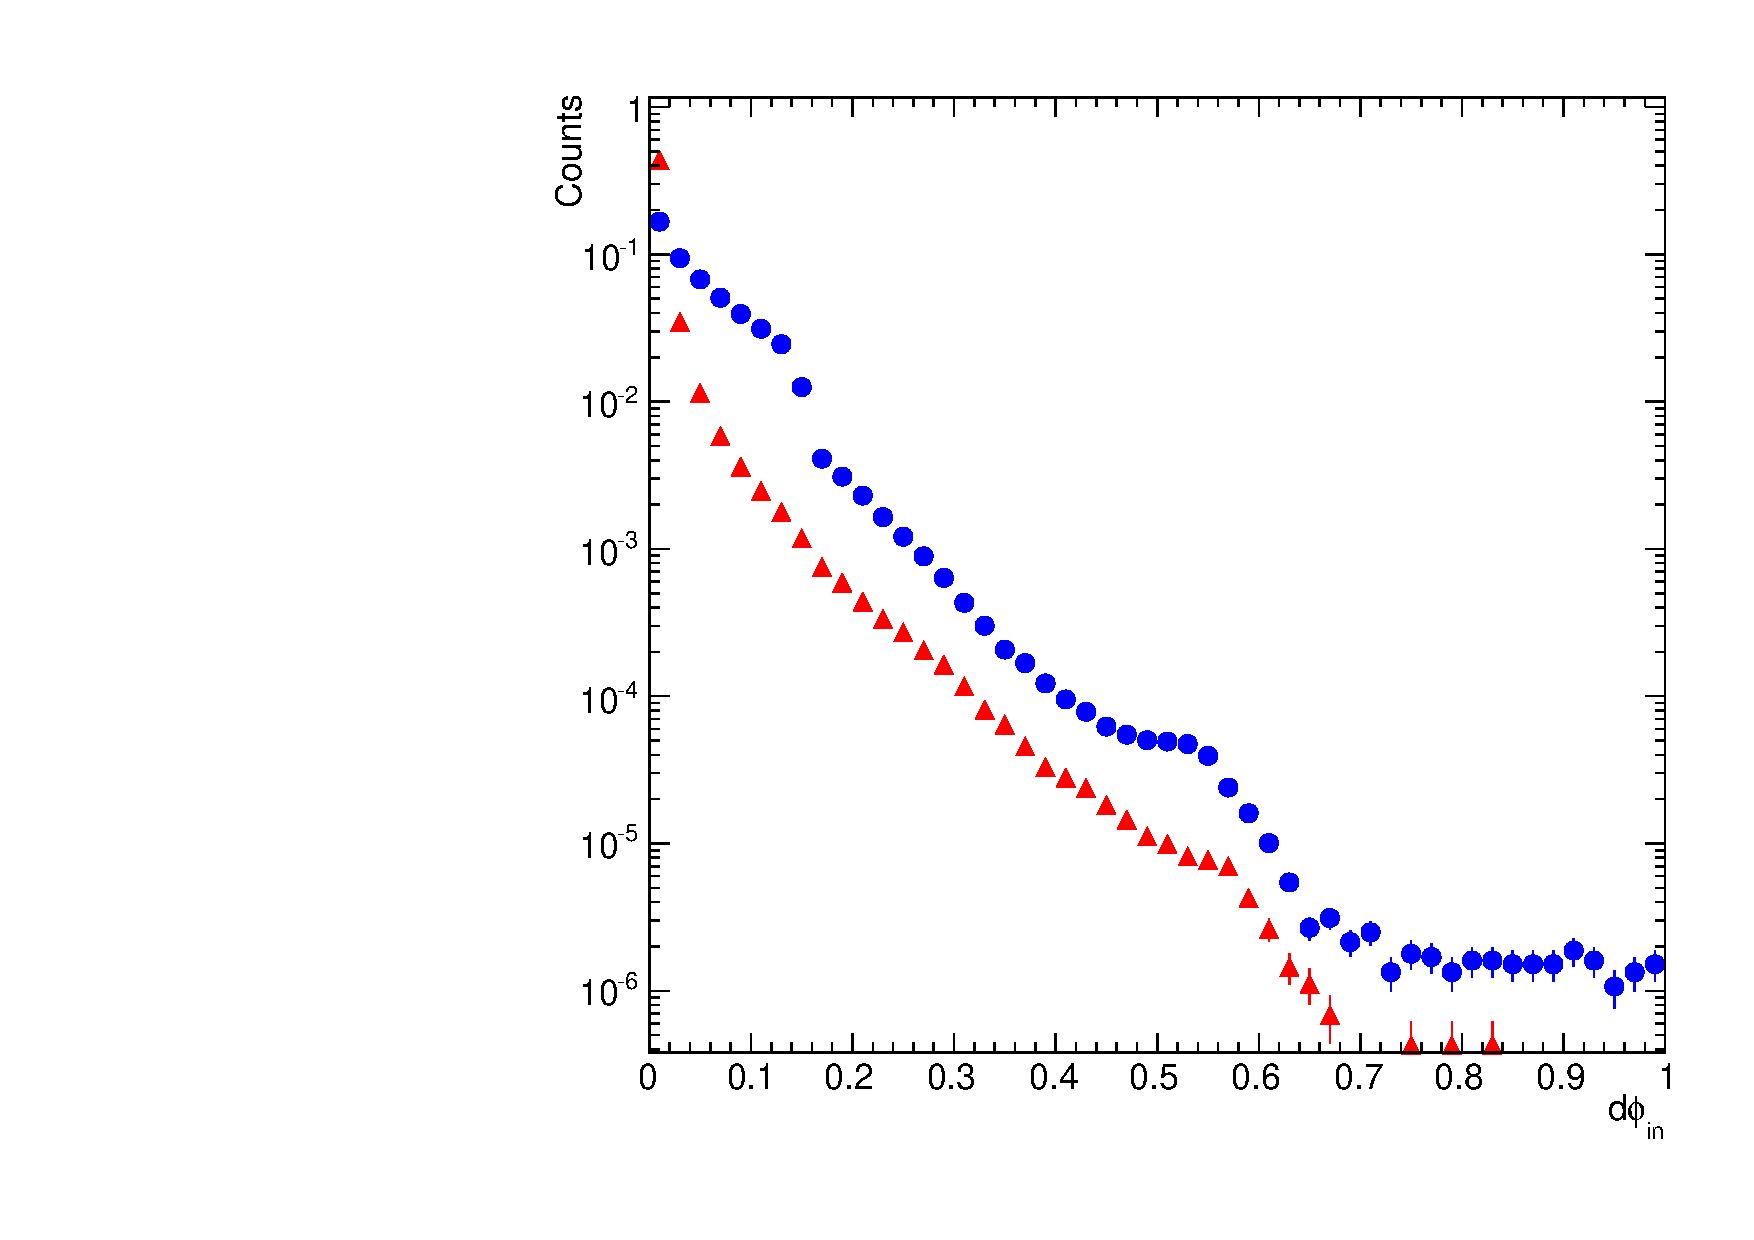
\includegraphics[width=\textwidth]{figures/dphi.pdf}
        \caption{}
        \label{fig:dphi}
    \end{subfigure}
    \caption[
        Distributions of $\detain$ and $\dphiin$ in data and MC.
    ]{
        The $\detain$ (top) and $\dphiin$ (bottom) variable distributions for
        all electrons with $\pt > 20 \GeV$ and $|\eta| < 2.4$ in a set of
        events selected with a muon trigger (circles) and in \MADGRAPH \Ztoee
        MC (triangles).
    }
    \label{fig:dtrack}
\end{figure}

\subsection{Conversion Rejection}

Conversions generally happen away from the vertex and so the distances of the
hits in the track from the vertex are useful quantities to reject conversions.
The transverse and longitudinal separation between the track and the primary
vertex are given by $d_{0}$ and $d_{z}$. Conversions generally happen deep in
the tracker and so tracks from them will have missing layers, given by \nmiss.
Conversions also have low vertex fit probability, \pvtx, indicating that their
track likely did not come from the primary vertex. A comparison of the
distributions of $d_{0}$ and of $d_{z}$ are shown in \FIGS~\ref{fig:d0} and
\ref{fig:dz}.

\begin{figure}[!htbp]
    \centering
    \begin{subfigure}[b]{0.65\textwidth}
        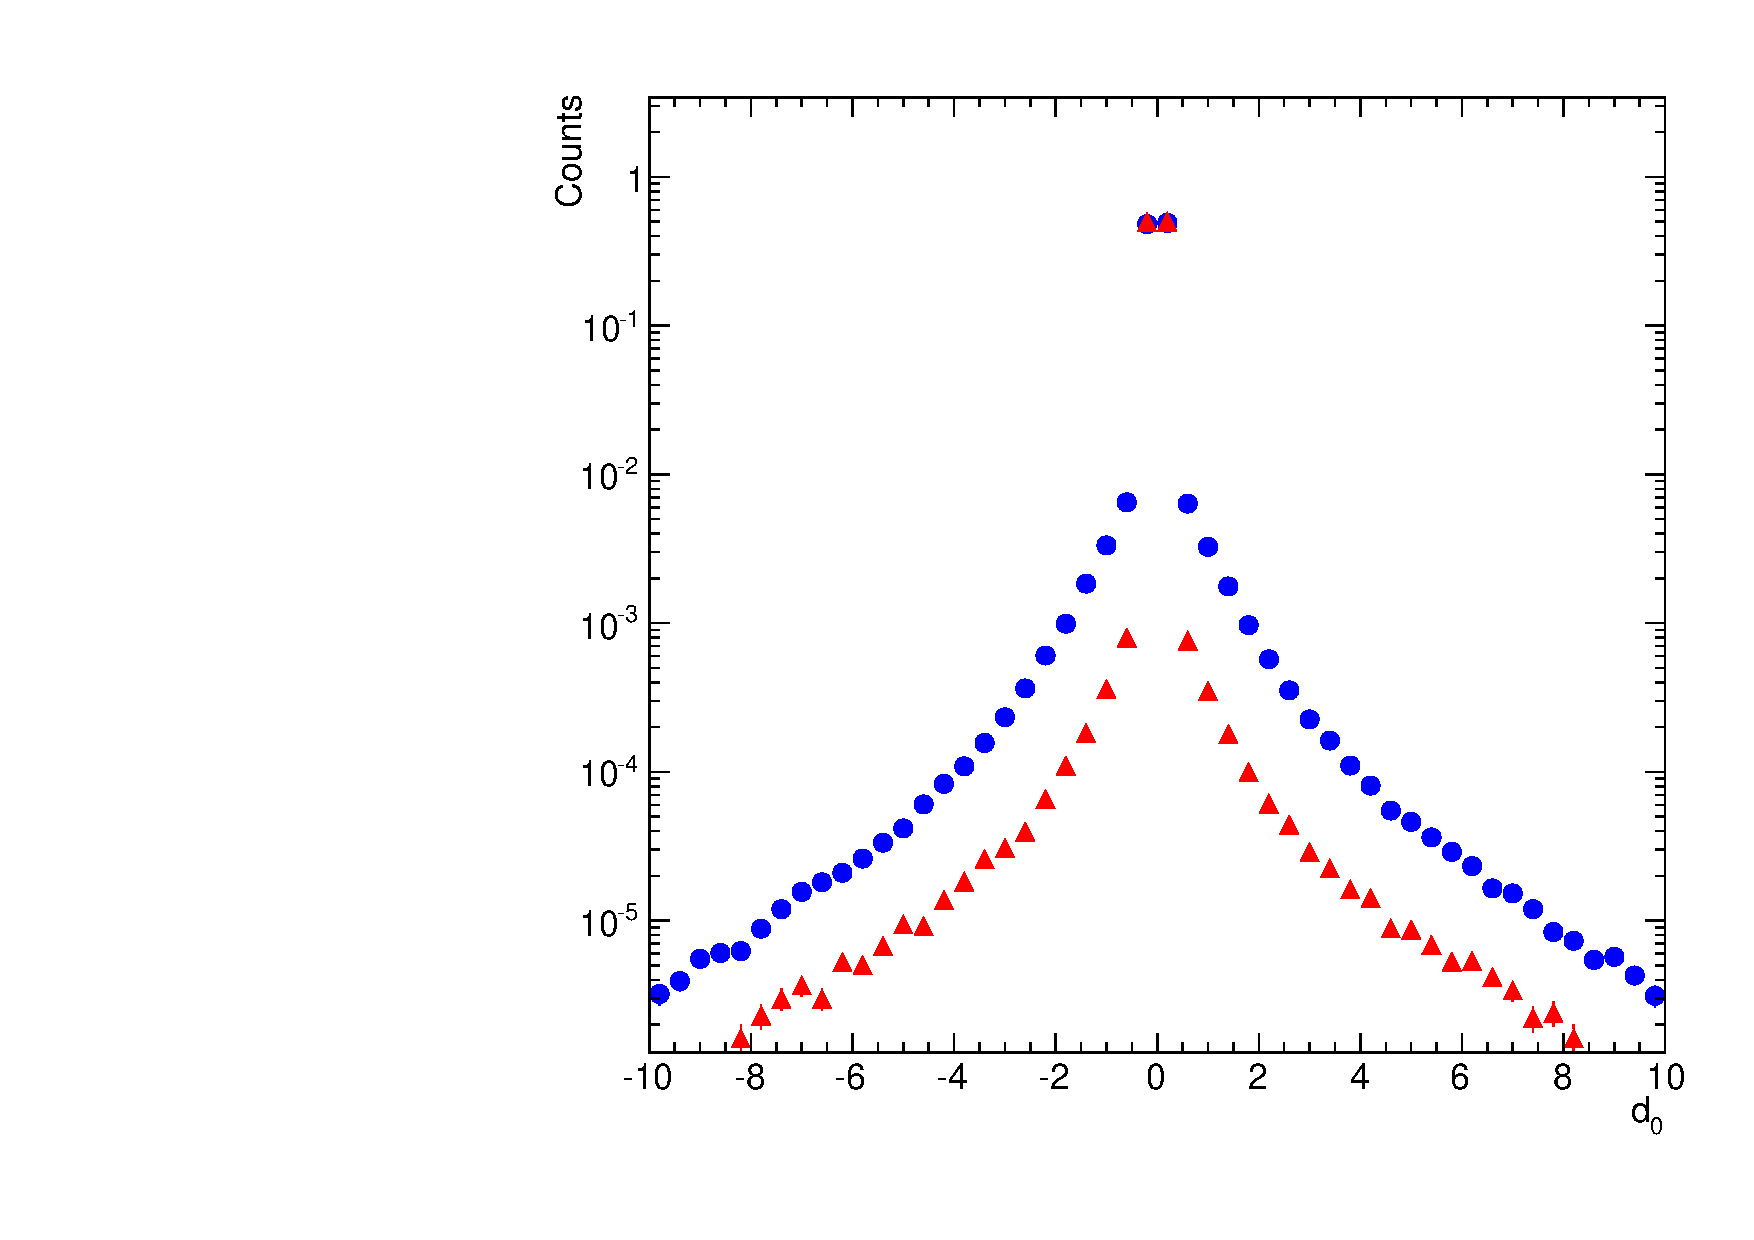
\includegraphics[width=\textwidth]{figures/d0.pdf}
        \caption{}
        \label{fig:d0}
    \end{subfigure}
    \begin{subfigure}[b]{0.65\textwidth}
        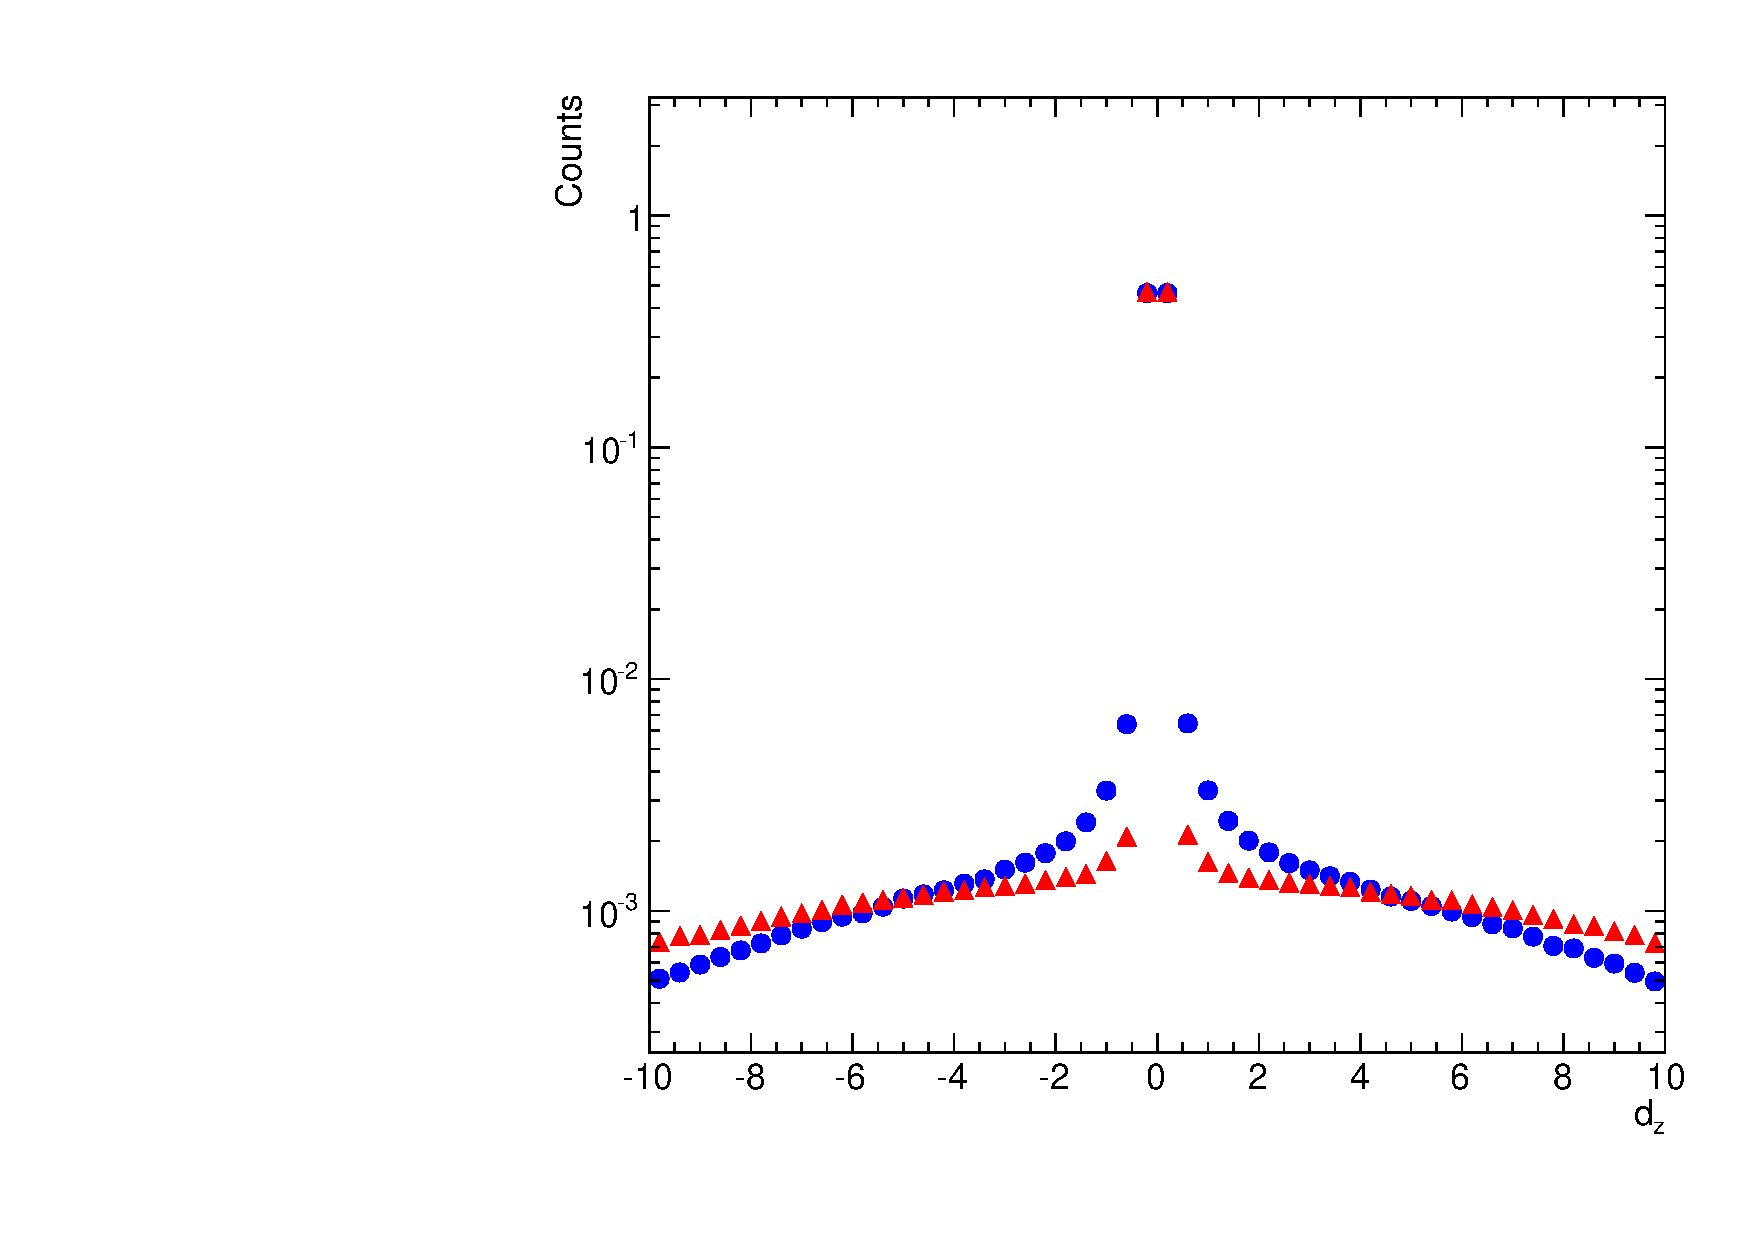
\includegraphics[width=\textwidth]{figures/dz.pdf}
        \caption{}
        \label{fig:dz}
    \end{subfigure}
    \caption[
        Distributions of $d_{0}$ and $d_{z}$ in data and MC.
    ]{
        The $d_{0}$ (top) and $d_{z}$ (bottom) variable distributions for all
        electrons with $\pt > 20 \GeV$ and $|\eta| < 2.4$ in a set of events
        selected with a muon trigger (circles) and in \MADGRAPH \Ztoee MC
        (triangles).
    }
    \label{fig:d0_dz}
\end{figure}
